\textbf{Finde benachbarte Dreiecke in einer Triangulierung}

Es sei $N \in \mathbb{N}$. Gegeben sei eine $N$ elementige Liste von Dreiecken $[\mathcal{T}_n]_{n\leq N}$, wobei jedes Dreieck definiert ist als Liste von Ecken $\mathcal{T}_n = [E_0, E_1, E_2 ]$ für $E_k \in \mathbb{N}$ (s. Bild). Zwei Dreiecke sind \textit{benachbart}, wenn sie genau zwei identische Ecken haben.
\begin{itemize}
	\item  Schreiben Sie eine Funktion \verb|N = neighbours(T)|, die eine Liste \texttt{T} von Dreiecken entgegennimmt und eine weitere Liste $\texttt{N}$ zurückgibt, die für jedes Dreieck die Nachbarn dieses Dreiecks enthält.
\end{itemize} 
Im Bild wäre dies eine Liste der Form $\texttt{N} = [[1,5], [0,2], \dots, [10,13]]$.
\begin{center}
	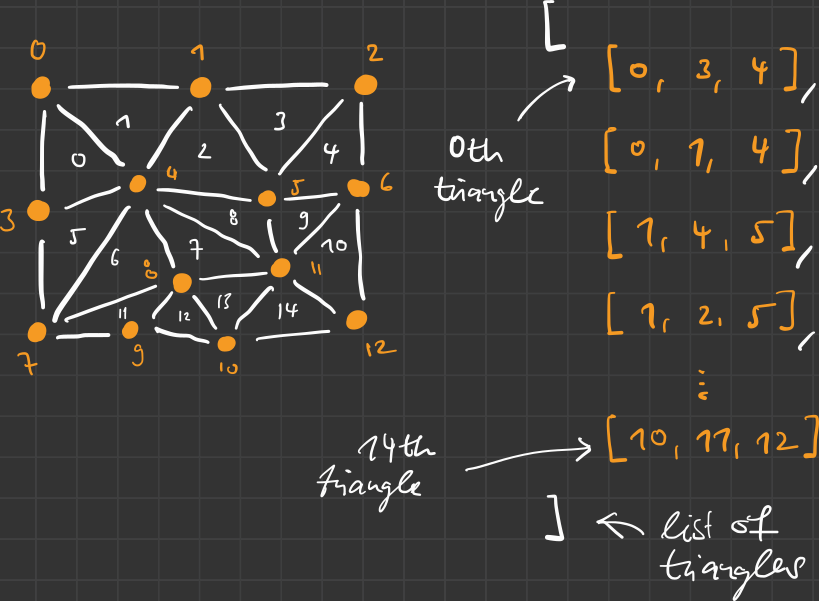
\includegraphics[scale=.8]{NeighbourCountTrianguation/example.png}
\end{center}
